\pagestyle{empty}

\begin{titlepage}
	
\begin{minipage}{\textwidth}
	\begin{center}
		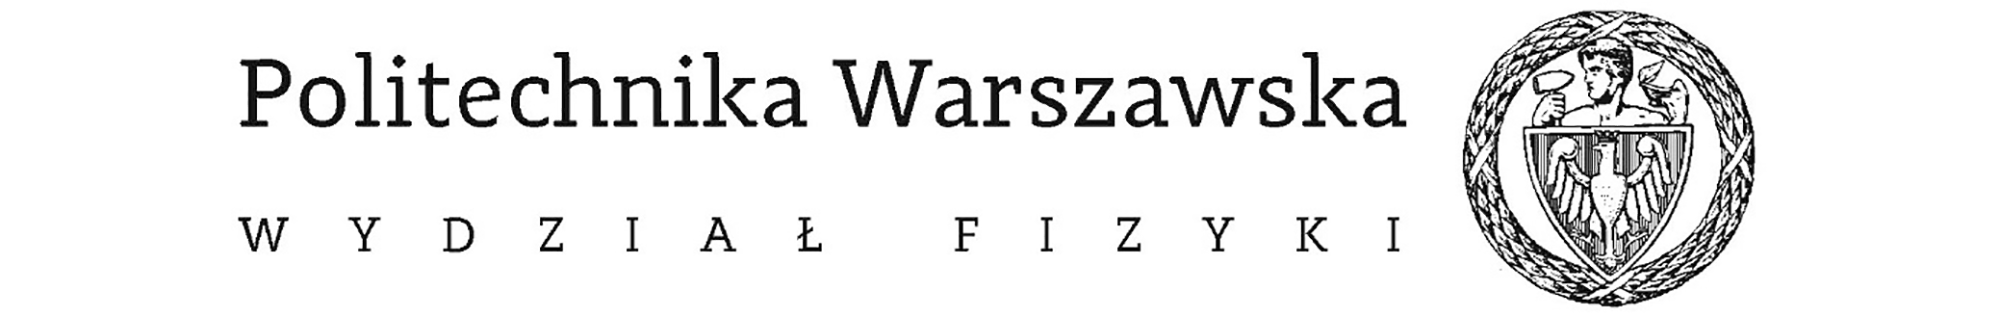
\includegraphics[width=\textwidth]{logo.png} \\
			\vspace{3cm}
		
\includegraphics[width=\textwidth]{inzynierska.png} \\ %podmieniæ na magisterska.png dla studiów II stopnia
			\vspace{1.5cm}
  			na kierunku fizyka techniczna \\
			w specjalności (specjalność) \\
			\vspace{2cm}	
		{\Large
			Tytuł pracy}

			\vspace{2cm}	
		{\huge
			Imię i nazwisko} \\
			Numer albumu: xxxxxx \\
			\vspace{1.5cm}	
			promotor: \\
			tytuł naukowy, imię i nazwisko \\
			\vspace{3cm}
			WARSZAWA 202x		
	\end{center}
\end{minipage}

\end{titlepage}

\newpage
\mbox{ }

\newpage
{\large \textbf{Streszczenie}}\\
{\color{sliwka}\rule[1pt]{\textwidth}{1.5pt}}

\begin{description}[leftmargin=2.2cm,font=\normalfont]
\item[Tytuł pracy:]  Tytuł
\end{description}

Streszczenie



\begin{flushright}
	Imię i nazwisko
\end{flushright}

\vspace{0.025\textheight}
\textit{sloowa kluczowe:}\\
\textit{szablon, LaTeX, praca dyplomowa}


\vspace{2cm}

\begin{multicols}{2}
	\begin{flushleft}
		(podpis opiekuna naukowego)
	\end{flushleft}
	\begin{flushright}
		(podpis dyplomanta)
	\end{flushright}
\end{multicols}

\newpage
\mbox{ }
\newpage
{\large \textbf{Abstract}}\\
{\color{sliwka}\rule[1pt]{\textwidth}{1.5pt}}


\begin{description}[leftmargin=3.2cm,font=\normalfont]
\item[Title of the thesis:] Title
\end{description}

Abstract



\vspace{0.025\textheight}
\textit{Keywords:}\\
\textit{template, LaTeX, thesis}


\newpage
\mbox{ }

\newpage
{\large \textbf{Oświadczenie o samodzielności wykonania pracy}}\\
{\color{sliwka}\rule[1pt]{\textwidth}{1.5pt}}

\vspace{0.6cm}

\begin{figure}[h!]
	
\includegraphics[width=0.5\textwidth]{img/pw_logo_tekst.png}
\end{figure}

\vspace{0.6cm}
{\large imię i nazwisko}\\
nr indeksu\\
kierunek studiów\\

\begin{center}
	{\large \textbf{Oświadczenie}}
\end{center}

{\large Świadomy/-a odpowiedzialności karnej za składanie fałszywych zeznań oświadczam, że niniejsza praca dyplomowa została napisana przeze mnie samodzielnie, pod opieką kierującego pracą dyplomową.}


Jednocześnie oświadczam, że:
\begin{itemize}
	\item niniejsza praca dyplomowa nie narusza praw autorskich w rozumieniu ustawy z dnia 4 lutego 1994 roku o prawie autorskim i prawach pokrewnych (Dz.U. z 2006 r. Nr 90, poz. 631 z późn. zm.) oraz dóbr osobistych chronionych prawem cywilnym,
	\item niniejsza praca dyplomowa nie zawiera danych i informacji, które uzyskałem/-am w sposób niedozwolony,
	\item niniejsza praca dyplomowa nie była wcześniej podstawą żadnej innej urzędowej procedury związanej z nadawaniem dyplomów lub tytułów zawodowych,
	\item wszystkie informacje umieszczone w niniejszej pracy, uzyskane ze źródeł pisanych i elektronicznych, zostały udokumentowane w wykazie literatury odpowiednimi odnośnikami,
	\item znam regulacje prawne Politechniki Warszawskiej w sprawie zarządzania prawami autorskimi i prawami pokrewnymi, prawami własności przemysłowej oraz zasadami komercjalizacji.
\end{itemize}

\vspace{3cm}

\begin{multicols}{2}
	\begin{flushleft}
		Warszawa, dnia (data)
	\end{flushleft}
	\begin{flushright}
		(czytelny podpis dyplomanta)
	\end{flushright}
\end{multicols}

\newpage
\mbox{ }

\newpage
{\large \textbf{Oświadczenie o udzieleniu Uczelni licencji do pracy}}\\
{\color{sliwka}\rule[1pt]{\textwidth}{1.5pt}}

\vspace{0.6cm}

\begin{figure}[h]
	
\includegraphics[width=0.5\textwidth]{img/pw_logo_tekst.png}
\end{figure}

\vspace{0.6cm}
{\large imię i nazwisko}\\
nr indeksu\\
kierunek studiów\\

\begin{center}
	{\large \textbf{Oświadczenie studenta w przedmiocie udzielenia licencji Politechnice Warszawskiej}}
\end{center}


Oświadczam, że jako autor / współautor* pracy dyplomowej pt.
\begin{center}
\textit{Tytuł pracy}
\end{center}
udzielam / nie udzielam* Politechnice Warszawskiej nieodpłatnej licencji na niewyłączne, nieograniczone w czasie, umieszczenie pracy dyplomowej w elektronicznych bazach danych oraz udostępnianie pracy dyplomowej w zamkniętym systemie bibliotecznym Politechniki Warszawskiej osobom zainteresowanym.
Licencja na udostępnienie pracy dyplomowej nie obejmuje wyrażenia zgody na wykorzystywanie pracy dyplomowej na żadnym innym polu eksploatacji, w szczególności kopiowania pracy dyplomowej w całości lub w części, utrwalania w innej formie czy zwielokrotniania.

\vspace{3cm}

\begin{multicols}{2}
	\begin{flushleft}
		Warszawa, dnia (data)
	\end{flushleft}
	\begin{flushright}
		(czytelny podpis dyplomanta)
	\end{flushright}
\end{multicols}
* - niepotrzebne skreślić

\newpage
\mbox{ }

